\section{Introduction}

The number of books published in the U.S. has been on the rise for at least the past decade, only incurring a small setback in 2005\cite{bowker}.
In 2010, Bowker recorded 328,259 new books published in the United States---up from 302,410 during the previous year.
Despite concerns that the paper book is on its way out, the book publishing industry is still very much a growing one.

% New Books Published per Year Graph
\begin{figure}
\begin{center}
\label{fig:new-books}
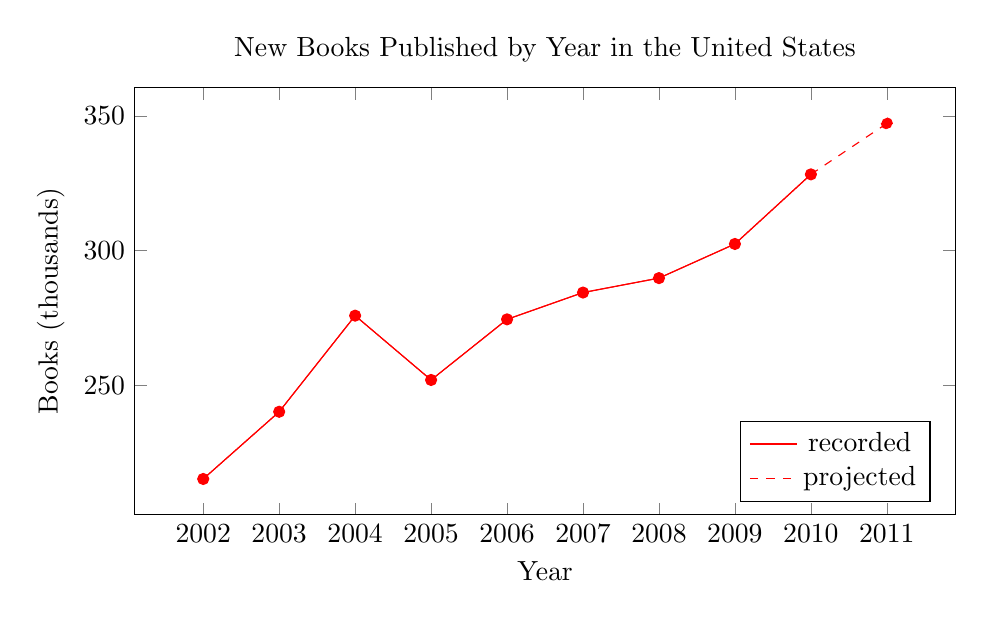
\begin{tikzpicture}
	\begin{axis}[
		title={New Books Published by Year in the United States},
		xlabel={Year},
		xticklabel style={/pgf/number format/1000 sep=},
		ylabel={Books (thousands)},
		width=12cm,
		height=7cm,
		legend pos=south east]
		
		\addplot[color=red,mark=,line join=round, solid] coordinates {
			(2002,215.138)
			(2003,240.098)
			(2004,275.793)
			(2005,251.903)
			(2006,274.416)
			(2007,284.370)
			(2008,289.729)
			(2009,302.410)
			(2010,328.259)
		};
		\addplot[color=red,mark=,line join=round, dashed] coordinates {
			(2010,328.259)
			(2011,347.178)
		};
		\addplot[color=red,mark=*,line join=round, solid] coordinates {
			(2002,215.138)
			(2003,240.098)
			(2004,275.793)
			(2005,251.903)
			(2006,274.416)
			(2007,284.370)
			(2008,289.729)
			(2009,302.410)
			(2010,328.259)
		};
		\addplot[color=red,mark=*,line join=round, dashed] coordinates {
			(2011,347.178)
		};
		
		\addlegendentry{recorded}
		\addlegendentry{projected}
	\end{axis}
\end{tikzpicture}
\caption{Publication statistics for traditional books published in the U.S.\cite{bowker}}.
\end{center}
\end{figure}

It's a fair assumption that many of these new books also contain an index section between their covers.
An index, of course, is, ``An alphabetical list, placed (usually) at the end of a book, of the names, subjects, etc. occurring in it, with indication of the places in which they occur,'' \cite{oed-index}.
Indexes are popular in non-fiction books, particularly in textbooks.
Readers use indexes to quickly and efficiently locate passages of the book focusing on a specific topic.
Thus, it is important for a book's index to be of high quality, so the reader can locate a particular topic with ease.
A good index can make learning and research easy, while a bad index can result in readers' frustration as they scan over each page in an attempt to find what they are looking for.

\subsection{Cost of Indexing}

The growing number of books published each year and the need for quality indexes in books of all types makes indexing an important sub-industry of the publication process.
Since many books contain indexes, any change in the indexing industry directly affects the publication industry.
If indexing could be made more efficient, the publishing industry could allocate the significant resources that would have gone toward indexing to other, more productive areas.

In {\it Indexing Books}, Nancy Mulvany estimates that an index for a 300 page book would cost approximately \$1,200.
This was in 2005.
Mulvany goes on to estimate the typical price-per-page at 4--6 2005 U.S. dollars\cite{mulvany}.
These prices are typically related to not only the number of pages, but also the amount of text on each page and the complexity of the topic.

In order to calculate the approximate cost of indexing the 328,259 new books published in 2010, it is also important to know that approximately 47\% of all books have indexes, and that the average indexed book is 380 pages long.
These data were found by recording page length and index information for 77 books from a random book generator using Amazon's product database. For more information on these numbers, see Appendix~\ref{appendix:d}.

\begin{center}
\begin{tabular}{|c|l|l|}
\hline
\multicolumn{1}{|c|}{{\bf Symbol}} & \multicolumn{1}{c|}{{\bf Description}} & \multicolumn{1}{c|}{{\bf Statistic}} \\
\hline
$b$ & Number of books published in 2010 \cite{bowker} & 328,259 books \\
\hline
$c$ & Percentage of Books requiring Indexes (see appx.~\ref{appendix:d}) & 47\% \\
\hline
$d$ & Average dollars per page indexed \cite{mulvany} & \$5 \\
\hline 
$p$ & Average Number of Pages in Book (see appx.~\ref{appendix:d}) & 380 pgs) \\ 
\hline 
$r$ & Average Number of Pages Indexed per Hour \cite{connolly} & 7 pgs/hr \\
\hline
\end{tabular}
\end{center}

Given these variables, equations are developed to calculate average cost and time impact of manual indexing.

\begin{figure}[H]
$$ \text{cost} = b \times c \times p \times d $$

$$ \text{time} = \frac{b \times c \times p}{r} $$

$$ 300,000,000 \text{ USD} = 328259 \times 0.47 \times 380 \times 5 $$

$$ 1000 \text{ years} = 8,000,000 \text{ hours} = \frac{328259 \times 0.47 \times 380}{7}$$
\caption{The Price of Manual Indexing}
\end{figure}

An estimate generated using these numbers reveals that over 300 million dollars were spent on indexing books in 2010. Work hours spent creating indexes is also revealing.
Using a professional indexer's average rate of 7 pages per hour, a similar calculation estimates that over 8 million work hours were spent creating indexes for 2010's new books. It would take a single person 380 years of indexing non-stop.

These numbers reveal the economic impact of indexing, but the individual impact is important too.
If an author wants to index his or her own book, it would take about 42 hours on average. The author could devote an entire work week towards something more productive if there existed an easier way to generate an index.
Clearly, indexing is a significant part of the publishing industry.
Computer software might be able to reduce these high costs, but first it is important to understand the indexing process before using technology to emulate it.

\subsection{Indexing Methods}
\label{sec:indexing-methods}

Historically, indexing was all done by hand without the assistance of technology beyond a stack of 3'' x 5'' note cards and a pen.
The ``index card'' method, as it is called, has the indexer create a separate index card for each word or phrase that appears in the index.
These note cards are created on the first pass through the document being indexed, and then they are organized alphabetically.
On the next and subsequent passes, the indexer combs the text looking for references to the words and phrases generated on the first pass, and records the page number of each occurrence on the appropriate note card.
At the end of this process, the selection of words and phrases is edited and then typeset \cite{mulvany}.
While this old fashioned method worked in the many years before computers became the powerful productivity tools they are today, computers now help indexers by providing purpose-built software that, in effect, replaces the paper note cards with a more efficient digital representation.

The author of {\it Indexing Books} describes computer-aided indexing by breaking indexing software used into major two types: embedded and dedicated.
Embedded indexing software helps a writer or an indexer mark, in the electronic text itself, the words and phrases that he or she wants to be indexed \cite{mulvany}.
Examples of embedded indexing software are Microsoft Word \cite{ms-word-indexing} and \LaTeX \cite{lamport}.
Dedicated indexing software, on the other hand, only provides tools whose purpose is to make creating an index easier, like the ability to digitize entries, sort them, and structure them in different ways\cite{mulvany}.
Dedicated software is different from embedded because dedicated does not allow the user to modify or display the full text of the work itself, instead focusing only on the index.
Examples of dedicated software are Macrex\cite{macrex} and SKY Index Professional\cite{sky-software}.
While these two types of software help indexers generate indexes, the indexer still performs a majority of the work of finding what ought to be indexed.
Even with today's computer-aided indexing software, the process of creating an index is still very much a manual one.

Automatic indexing is the lesser known third type of indexing software, and it is the subject of this research.
Mulvany defines automatic indexing software as that which, ``conjures up images of indexing at the push of a button, the computer taking care of all the drudgery and the thinking involved in creating an index''\cite{mulvany}.
Although she recognizes it as a computer science research focus, she does not think highly of present-day automatic indexing, stating that, ``There is nothing automatic about the index-writing process.
There is no automatic indexing tool available that could produce the index in the back of this book''\cite{mulvany}.
Given the career implications of automatic indexing on indexing professionals, it is unsurprising that Mulvany is skeptical.
However, for the most part she is correct: current software does not perform as well as humans at the task of indexing a book.
If it did perform better than humans, then publishers and authors would be purchasing the software rather than hiring indexers.

The goal of this research is to further the knowledge of automatic indexing by applying techniques from Natural Language Processing (NLP), a subfield of Computer Science that concerns itself with teaching computers to understand language mechanics.
